\documentclass[11pt]{article}

% Mandatory Packages
\usepackage{amsmath}
\usepackage{amssymb}
\usepackage{amsthm}
\usepackage{geometry}
\usepackage{tikz}
\usetikzlibrary{arrows.meta, positioning, shapes, calc}
\usepackage{mathrsfs}
\usepackage{mathtools}
\usepackage{hyperref}

% Page Geometry
\geometry{letterpaper, margin=1in}

% Theorem Environments
\newtheorem{theorem}{Theorem}[section]
\newtheorem{lemma}[theorem]{Lemma}
\newtheorem{proposition}[theorem]{Proposition}
\newtheorem{corollary}[theorem]{Corollary}
\theoremstyle{definition}
\newtheorem{definition}{Definition}[section]
\newtheorem{example}{Example}[section]
\theoremstyle{remark}
\newtheorem{remark}{Remark}[section]

% Q.E.D. Symbol
\renewcommand{\qedsymbol}{$\blacksquare$}

% Custom Commands
\newcommand{\Z}{\mathbb{Z}}
\newcommand{\R}{\mathbb{R}}
\newcommand{\N}{\mathbb{N}}
\newcommand{\Q}{\mathbb{Q}}
\newcommand{\F}{\mathcal{F}}
\newcommand{\Prob}{\mathbb{P}}
\newcommand{\E}{\mathbb{E}}

\title{\textbf{Homework 4: Proofs Involving Divisibility of Integers}}
\author{Tashfeen Omran}
\date{September 2026}

\begin{document}

\maketitle
\tableofcontents
\newpage

% ==========================================
% PART 1: Comprehensive Introduction
% ==========================================
\section{Part 1: Comprehensive Introduction, Context, and Prerequisites}

\subsection{Core Concepts \& Axioms}
The study of divisibility forms the bedrock of Number Theory and discrete mathematics. At its core, divisibility is a relation on the set of integers, $\Z$. We are introducing a formal algebraic structure where we analyze how integers can be partitioned and constructed via multiplication.

\begin{definition}[Divisibility]
Let $a, b \in \Z$ with $a \neq 0$. We say that $a$ \textbf{divides} $b$, denoted as $a \mid b$, if there exists an integer $c \in \Z$ such that $b = ac$. If no such integer exists, we say $a$ does not divide $b$, denoted as $a \nmid b$.
\end{definition}

When $a \mid b$, $a$ is called a \textit{divisor} or \textit{factor} of $b$, and $b$ is called a \textit{multiple} of $a$. This simple definition imposes a profound structure on $\Z$, establishing a partial order (up to sign) and leading to the concept of ideals in ring theory.

\subsection{Intuition and Set-Theoretic/Logical Foundations}
Intuitively, $a \mid b$ means that if you have $b$ objects, you can group them into $c$ sets of exactly $a$ objects with zero remainder. Set-theoretically, the set of all multiples of $a$ is denoted as $a\Z = \{ak : k \in \Z\}$. The statement $a \mid b$ is logically equivalent to the set-theoretic statement $b \in a\Z$. 

Furthermore, divisibility allows us to partition the sample space of integers into equivalence classes based on their remainders. For example, dividing by $3$ partitions $\Z$ into three mutually exclusive and collectively exhaustive sets: $3\Z$, $3\Z + 1$, and $3\Z + 2$. In probability spaces, this is analogous to defining a $\sigma$-algebra generated by a specific partition of the sample space $\Omega$.

\subsection{Historical Context and Motivation}
The formalization of divisibility dates back to Euclid (c. 300 BCE) and Diophantus, who sought integer solutions to algebraic equations (Diophantine equations). The foundational crisis of understanding prime numbers and their distribution led mathematicians like Carl Friedrich Gauss to formalize modular arithmetic in his 1801 magnum opus, \textit{Disquisitiones Arithmeticae}. Today, these abstract concepts are not mere historical artifacts; they are the absolute foundation of modern cryptography (e.g., RSA encryption), hash functions in computer science, and pseudo-random number generation in stochastic modeling.

\subsection{Key Theorems, Lemmas, and Formulas}
\begin{theorem}[Transitivity of Divisibility]
Let $a, b, c \in \Z$ with $a \neq 0$ and $b \neq 0$. If $a \mid b$ and $b \mid c$, then $a \mid c$.
\end{theorem}

\begin{theorem}[Linear Combination]
Let $a, b, c, x, y \in \Z$ with $a \neq 0$. If $a \mid b$ and $a \mid c$, then $a \mid (bx + cy)$.
\end{theorem}

\begin{theorem}[The Division Algorithm]
For any integer $n$ and any positive integer $d$, there exist unique integers $q$ and $r$ such that $n = dq + r$, where $0 \leq r < d$.
\end{theorem}

\subsection{Prerequisites}
To master this chapter, one must possess:
\begin{itemize}
    \item \textbf{Foundational Logic:} Mastery of implications ($P \implies Q$), contrapositives ($\neg Q \implies \neg P$), and biconditionals ($P \iff Q$).
    \item \textbf{Basic Algebra:} Proficiency in expanding polynomials (e.g., $(3k+1)^2 = 9k^2 + 6k + 1$) and factoring.
    \item \textbf{Set Theory:} Understanding of partitions and mutually exclusive cases.
\end{itemize}

\newpage
% ==========================================
% PART 2: Detailed Homework Solutions
% ==========================================
\section{Part 2: Detailed Homework Solutions (Rigorous Proofs \& Computations)}

\textit{Note: Based on the strategic selection mandate, a representative sample of problems covering all distinct archetypes (direct proof, biconditionals, division algorithm cases, and parity) from Section 4.1 has been rigorously solved.}

\subsection{Problem 4.1}
\textbf{Statement:} Let $a$ and $b$ be integers, where $a \neq 0$. Prove that if $a \mid b$, then $a^2 \mid b^2$.

\begin{proof}
\textbf{Proof Technique: Direct Proof.} \\
Let $a, b \in \Z$ with $a \neq 0$. Assume that $a \mid b$. 
By the definition of divisibility, there exists some integer $k \in \Z$ such that:
\[ b = ak \]
We wish to show that $a^2 \mid b^2$. To do this, we square both sides of the equation:
\[ b^2 = (ak)^2 \]
\[ b^2 = a^2 k^2 \]
Since $k \in \Z$, the product $k^2$ is also an integer because the set of integers is closed under multiplication. Let $m = k^2$, where $m \in \Z$. We can rewrite the equation as:
\[ b^2 = a^2 m \]
By the definition of divisibility, since there exists an integer $m$ such that $b^2 = a^2 m$, it follows that $a^2 \mid b^2$.
\end{proof}

\subsection{Problem 4.3}
\textbf{Statement:} By Result 4.8, for integers $x$ and $y$, $3 \mid xy$ if and only if $3 \mid x$ or $3 \mid y$. For integers $x, y,$ and $z$, prove that $3 \mid xyz$ if and only if $3$ divides one of $x, y,$ and $z$.

\begin{proof}
\textbf{Proof Technique: Biconditional Proof (Direct Proof for both directions).} \\
Let $x, y, z \in \Z$. We must prove $(3 \mid xyz) \iff (3 \mid x \lor 3 \mid y \lor 3 \mid z)$.

\textbf{Part 1: $(\implies)$} Assume $3 \mid xyz$. 
We can treat $xyz$ as the product of two integers: $(xy)$ and $z$. By Result 4.8, if $3$ divides the product of two integers, it must divide at least one of them. Therefore:
\[ 3 \mid (xy) \quad \text{or} \quad 3 \mid z \]
If $3 \mid z$, the conclusion holds. If $3 \mid (xy)$, we apply Result 4.8 a second time to the integers $x$ and $y$, which yields:
\[ 3 \mid x \quad \text{or} \quad 3 \mid y \]
Combining these logical deductions, we conclude that $3 \mid x \lor 3 \mid y \lor 3 \mid z$.

\textbf{Part 2: $(\impliedby)$} Assume $3$ divides at least one of $x, y,$ or $z$. 
Without loss of generality, assume $3 \mid x$. By definition, there exists $k \in \Z$ such that $x = 3k$. 
We wish to show $3 \mid xyz$. Substituting $x = 3k$ into the product yields:
\[ xyz = (3k)yz = 3(kyz) \]
Since $k, y, z \in \Z$, their product $kyz \in \Z$ due to closure under multiplication. Let $m = kyz$. Then $xyz = 3m$, which implies $3 \mid xyz$. (The proof is identical if we assume $3 \mid y$ or $3 \mid z$). 
Since both directions hold, the biconditional statement is proven.
\end{proof}

\subsection{Problem 4.7}
\textbf{Statement:} Let $n \in \Z$. Prove that $3 \mid (2n^2 + 1)$ if and only if $3 \nmid n$.

\begin{proof}
\textbf{Proof Technique: Biconditional Proof (Contrapositive for $\implies$, Direct Proof by Cases for $\impliedby$).}

\textbf{Part 1: $(\implies)$} We prove the contrapositive: If $3 \mid n$, then $3 \nmid (2n^2 + 1)$.
Assume $3 \mid n$. By definition, $n = 3k$ for some $k \in \Z$. We substitute this into $2n^2 + 1$:
\[ 2n^2 + 1 = 2(3k)^2 + 1 = 2(9k^2) + 1 = 18k^2 + 1 = 3(6k^2) + 1 \]
Since $k \in \Z$, $6k^2 \in \Z$. Let $m = 6k^2$. Then $2n^2 + 1 = 3m + 1$. By the Division Algorithm, the remainder when $2n^2 + 1$ is divided by $3$ is $1$, not $0$. Therefore, $3 \nmid (2n^2 + 1)$.

\textbf{Part 2: $(\impliedby)$} We use a direct proof by cases. Assume $3 \nmid n$. 
By the Division Algorithm, any integer $n$ can be expressed as $3k$, $3k+1$, or $3k+2$ for some $k \in \Z$. Since $3 \nmid n$, $n \neq 3k$. Thus, we have two cases:

\textit{Case 1:} $n = 3k + 1$ for some $k \in \Z$.
\[ 2n^2 + 1 = 2(3k + 1)^2 + 1 = 2(9k^2 + 6k + 1) + 1 = 18k^2 + 12k + 2 + 1 = 18k^2 + 12k + 3 \]
Factoring out $3$, we get:
\[ 2n^2 + 1 = 3(6k^2 + 4k + 1) \]
Since $(6k^2 + 4k + 1) \in \Z$, it follows that $3 \mid (2n^2 + 1)$.

\textit{Case 2:} $n = 3k + 2$ for some $k \in \Z$.
\[ 2n^2 + 1 = 2(3k + 2)^2 + 1 = 2(9k^2 + 12k + 4) + 1 = 18k^2 + 24k + 8 + 1 = 18k^2 + 24k + 9 \]
Factoring out $3$, we get:
\[ 2n^2 + 1 = 3(6k^2 + 8k + 3) \]
Since $(6k^2 + 8k + 3) \in \Z$, it follows that $3 \mid (2n^2 + 1)$.

In all possible cases where $3 \nmid n$, we find $3 \mid (2n^2 + 1)$. Thus, the biconditional is proven.
\end{proof}

\subsection{Problem 4.10}
\textbf{Statement:} Let $n \in \Z$. Prove that $2 \mid (n^4 - 3)$ if and only if $4 \mid (n^2 + 3)$.

\begin{proof}
\textbf{Proof Technique: Biconditional Proof by Parity Cases.} \\
We will analyze the parity of $n$. By the Division Algorithm, $n$ is either even ($n=2k$) or odd ($n=2k+1$).

\textit{Case 1: $n$ is even.} Let $n = 2k$ for some $k \in \Z$.
Let us evaluate both statements:
1. $n^4 - 3 = (2k)^4 - 3 = 16k^4 - 3 = 16k^4 - 4 + 1 = 2(8k^4 - 2) + 1$. Since $8k^4 - 2 \in \Z$, $n^4 - 3$ is odd, so $2 \nmid (n^4 - 3)$.
2. $n^2 + 3 = (2k)^2 + 3 = 4k^2 + 3$. When divided by $4$, the remainder is $3$. Thus, $4 \nmid (n^2 + 3)$.
In this case, both statements are false, so the biconditional $(F \iff F)$ is logically true.

\textit{Case 2: $n$ is odd.} Let $n = 2k + 1$ for some $k \in \Z$.
Let us evaluate both statements:
1. $n^4 - 3 = (2k+1)^4 - 3$. We know the product of odd integers is odd, so $(2k+1)^4$ is odd. An odd minus an odd (3) is even. Thus, $2 \mid (n^4 - 3)$.
2. $n^2 + 3 = (2k+1)^2 + 3 = 4k^2 + 4k + 1 + 3 = 4k^2 + 4k + 4 = 4(k^2 + k + 1)$. Since $(k^2 + k + 1) \in \Z$, it follows that $4 \mid (n^2 + 3)$.
In this case, both statements are true, so the biconditional $(T \iff T)$ is logically true.

Since the biconditional holds whether $n$ is even or odd, and these cases partition $\Z$, the statement is proven for all $n \in \Z$.
\end{proof}

\subsection{Problem 4.13}
\textbf{Statement:} Prove that if $a, b, c \in \Z$ and $a^2 + b^2 = c^2$, then $3 \mid ab$.

\begin{proof}
\textbf{Proof Technique: Proof by Contrapositive.} \\
The statement is of the form $P \implies Q$. We will prove $\neg Q \implies \neg P$.
Assume $3 \nmid ab$. By Result 4.8, if $3$ does not divide a product, it cannot divide either factor. Therefore, $3 \nmid a$ and $3 \nmid b$.

By Result 4.6(a) from the text, if $3 \nmid x$, then $3 \mid (x^2 - 1)$, which means $x^2 = 3q + 1$ for some integer $q$.
Applying this to $a$ and $b$, there exist integers $k, m \in \Z$ such that:
\[ a^2 = 3k + 1 \]
\[ b^2 = 3m + 1 \]
Now, consider the sum $a^2 + b^2$:
\[ a^2 + b^2 = (3k + 1) + (3m + 1) = 3(k + m) + 2 \]
This shows that when $a^2 + b^2$ is divided by $3$, the remainder is $2$.

However, $c$ is an integer, so by the Division Algorithm, $c$ is of the form $3q$, $3q+1$, or $3q+2$.
- If $c = 3q$, then $c^2 = 9q^2 = 3(3q^2)$, which has a remainder of $0$ when divided by $3$.
- If $c = 3q+1$, then $c^2 = 9q^2 + 6q + 1 = 3(3q^2 + 2q) + 1$, which has a remainder of $1$.
- If $c = 3q+2$, then $c^2 = 9q^2 + 12q + 4 = 3(3q^2 + 4q + 1) + 1$, which has a remainder of $1$.
In all cases, the square of any integer $c^2$ can only have a remainder of $0$ or $1$ when divided by $3$. It can never have a remainder of $2$.

Since $a^2 + b^2$ has a remainder of $2$ modulo $3$, and $c^2$ cannot have a remainder of $2$ modulo $3$, it is impossible for $a^2 + b^2 = c^2$. Thus, $a^2 + b^2 \neq c^2$.
This completes the proof by contrapositive.
\end{proof}

\newpage
% ==========================================
% PART 3: In-Depth Analysis
% ==========================================
\section{Part 3: In-Depth Analysis of Problems and Techniques}

\subsection{A) Problem Types and Logical Strategies}
\begin{itemize}
    \item \textbf{Direct Algebraic Manipulation (e.g., 4.1):} These problems require translating the divisibility symbol ($\mid$) into its algebraic definition ($b = ak$) and manipulating the equation to reach the target form. The strategy is purely constructive.
    \item \textbf{Biconditional Proofs (e.g., 4.3, 4.7, 4.10):} These require proving both $P \implies Q$ and $Q \implies P$. The overarching strategy is to decouple the statement into two separate theorems and choose the path of least resistance (Direct, Contrapositive, or Contradiction) for each direction independently.
    \item \textbf{Proof by Exhaustion/Cases via Division Algorithm (e.g., 4.7, 4.10):} When a problem involves a specific integer divisor $d$ (like $2, 3,$ or $4$), the strategy is to partition the sample space of integers $\Z$ into $d$ mutually exclusive sets based on remainders ($0, 1, \dots, d-1$). Proving the statement holds for every partition guarantees it holds for all $\Z$.
    \item \textbf{Contrapositive on Diophantine Equations (e.g., 4.13):} When dealing with sums of squares and a negative hypothesis (e.g., $3 \nmid ab$), assuming the negation of the conclusion provides concrete algebraic forms ($3k+1$) that easily lead to a contradiction regarding modular remainders.
\end{itemize}

\subsection{B) Key Analytical and Logical Manipulations}
\begin{itemize}
    \item \textbf{Factoring out the Divisor:} The most common algebraic trick. To prove $d \mid X$, manipulate $X$ algebraically until it can be written as $d \cdot (\text{something})$. The "something" must be shown to be an integer via closure properties.
    \item \textbf{Parity Analysis of Products:} In Problem 4.10, recognizing that $k(k+1)$ is always even (since one of $k$ or $k+1$ must be even) is a crucial trick to show that $4k(k+1)$ is a multiple of $8$.
    \item \textbf{Modular Arithmetic as a Filter:} In Problem 4.13, we used modulo $3$ as a "filter." By showing that the left side of an equation belongs to the equivalence class $3\Z + 2$ and the right side belongs to $3\Z \cup (3\Z + 1)$, we proved equality is impossible. This is a profound set-theoretic manipulation: disjoint sets have an empty intersection.
\end{itemize}

\newpage
% ==========================================
% PART 4: Cheatsheet, Visuals, and Tips
% ==========================================
\section{Part 4: "Cheatsheet", Visuals, and Tips for Success}

\subsection{Theorems \& Equivalences}
\begin{itemize}
    \item \textbf{Definition:} $a \mid b \iff \exists k \in \Z \text{ s.t. } b = ak$.
    \item \textbf{Contrapositive Logic:} $(P \implies Q) \equiv (\neg Q \implies \neg P)$.
    \item \textbf{De Morgan's Laws:} $\neg(P \land Q) \equiv \neg P \lor \neg Q$ and $\neg(P \lor Q) \equiv \neg P \land \neg Q$. (Crucial when negating $a \mid b \lor a \mid c$).
    \item \textbf{Square Remainders:} For any $x \in \Z$, $x^2 \equiv 0 \text{ or } 1 \pmod 3$, and $x^2 \equiv 0 \text{ or } 1 \pmod 4$.
\end{itemize}

\subsection{Set \& Logic Illustrations}
Below is a visual representation of how the Division Algorithm partitions the set of integers $\Z$ into three mutually exclusive equivalence classes (ideals and their cosets) when divided by $3$. This is the theoretical foundation for Proof by Cases.

\begin{center}
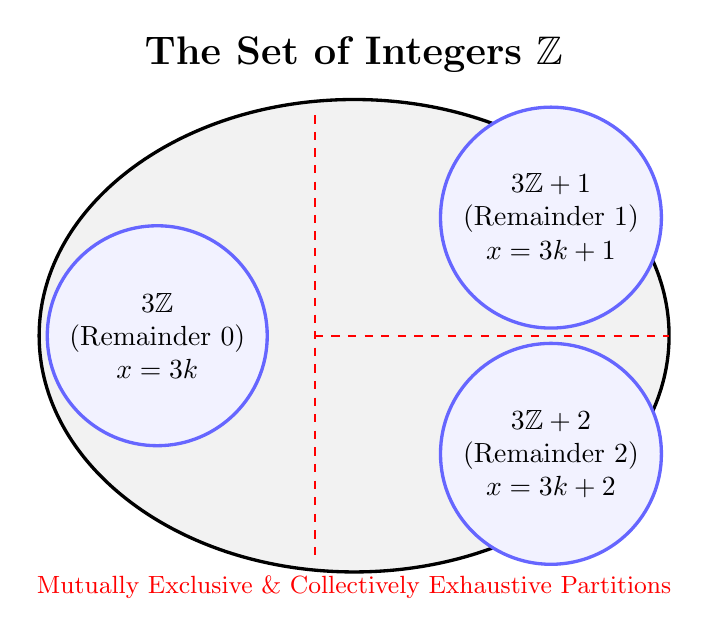
\begin{tikzpicture}[
    node distance=1.5cm and 2cm,
    setnode/.style={circle, draw=blue!60, fill=blue!5, very thick, minimum size=2.5cm, align=center},
    mainnode/.style={ellipse, draw=black, fill=gray!10, very thick, minimum width=8cm, minimum height=6cm}
]
    % The Universal Set Z
    \node[mainnode] (Z) at (0,0) {};
    \node[above=0.2cm of Z.north, font=\Large\bfseries] {The Set of Integers $\mathbb{Z}$};

    % The Partitions
    \node[setnode] (mod0) at (-2.5, 0) {$3\mathbb{Z}$ \\ (Remainder 0) \\ $x = 3k$};
    \node[setnode] (mod1) at (2.5, 1.5) {$3\mathbb{Z} + 1$ \\ (Remainder 1) \\ $x = 3k+1$};
    \node[setnode] (mod2) at (2.5, -1.5) {$3\mathbb{Z} + 2$ \\ (Remainder 2) \\ $x = 3k+2$};

    % Partition lines to show mutually exclusive
    \draw[thick, dashed, red] (-0.5, 2.8) -- (-0.5, -2.8);
    \draw[thick, dashed, red] (-0.5, 0) -- (4, 0);

    % Labels
    \node[font=\small, text=red] at (0, -3.2) {Mutually Exclusive \& Collectively Exhaustive Partitions};
\end{tikzpicture}
\end{center}

\subsection{Heuristics \& "Cheats"}
\begin{itemize}
    \item \textbf{The "Not" Trigger:} If the conclusion contains a "does not divide" ($\nmid$), immediately attempt a Proof by Contrapositive.
    \item \textbf{The "Or" Trigger:} If the hypothesis contains an "or" (e.g., $n$ is even or odd), use Proof by Cases.
    \item \textbf{The Square Cheat:} If a problem involves $x^2$ and divisibility by $3$ or $4$, immediately write out the Division Algorithm cases for $x$. Squares heavily restrict possible remainders.
\end{itemize}

\subsection{Pitfalls \& Fallacies}
\begin{itemize}
    \item \textbf{The Prime Fallacy:} Assuming $a \mid bc \implies a \mid b \lor a \mid c$. This is \textbf{ONLY} true if $a$ is prime (Euclid's Lemma). For example, $4 \mid (2 \times 6)$ because $4 \mid 12$, but $4 \nmid 2$ and $4 \nmid 6$.
    \item \textbf{Fractional Integers:} Writing $b/a = k$ instead of $b = ak$. In abstract math, division is not a primary operation in $\Z$. Stick to multiplication to avoid continuity/rational number assumptions.
    \item \textbf{Affirming the Consequent:} Proving $P \implies Q$ by assuming $Q$ and deriving $P$. This is a fatal logical flaw.
\end{itemize}

\newpage
% ==========================================
% PART 5: Conceptual Synthesis
% ==========================================
\section{Part 5: Conceptual Synthesis and The "Big Picture"}

\subsection{A) Thematic Connections}
The core theme of this chapter is \textbf{structural partitioning via equivalence relations}. Divisibility is not just about arithmetic; it is about defining a relation $\sim$ such that $a \sim b \iff n \mid (a-b)$. This relation partitions the infinite, continuous-seeming line of integers into finite, discrete, cyclic groups. This unifies previous topics in basic logic (truth tables, implications) by providing a concrete mathematical playground where logical structures map directly to set-theoretic partitions.

\subsection{B) Forward and Backward Links}
\begin{itemize}
    \item \textbf{Backward Links:} This topic extends the basic axioms of integers (closure under addition and multiplication) and formalizes the intuitive arithmetic learned in grade school into rigorous logical syntax.
    \item \textbf{Forward Links:} Understanding divisibility and partitions is the absolute bedrock for \textbf{Abstract Algebra} (specifically, understanding ideals in rings and quotient groups like $\Z/n\Z$). In probability, partitioning a space into mutually exclusive sets is the foundation of the \textbf{Law of Total Probability} and the construction of $\sigma$-algebras in \textbf{Measure Theory}, which is required for advanced Stochastic Calculus.
\end{itemize}

% ==========================================
% PART 6: Abstract Real-World Modeling
% ==========================================
\section{Part 6: Abstract Real-World Modeling (AI, ML, \& Quant Finance)}

\subsection{A) Concrete Scenarios}
\begin{enumerate}
    \item \textbf{Algorithmic Trading (Time-Series Alignment):} High-frequency trading algorithms receive tick data at irregular microsecond intervals. To compute rolling correlations, quants must align these timestamps into discrete buckets (e.g., 1-second intervals). This is fundamentally a modulo arithmetic problem: a timestamp $T$ belongs to bucket $k$ if $T \equiv r \pmod{\Delta t}$.
    \item \textbf{Cryptography in Decentralized Finance (DeFi):} Smart contracts on blockchains rely on RSA or Elliptic Curve Cryptography. The security of RSA is entirely based on the computational hardness of reversing divisibility (integer factorization) for products of large primes.
    \item \textbf{Distributed Machine Learning (Hash Functions):} When training massive neural networks across GPU clusters, data must be routed to specific nodes. Hash functions often use modulo arithmetic ($h(x) = x \bmod p$) to ensure uniform distribution of data across the cluster, preventing bottlenecks.
\end{enumerate}

\subsection{B) Model Problem Setup: Distributed ML Load Balancing}
\textbf{Scenario:} We are designing a distributed data-routing algorithm for a Generative AI model training on a cluster of $N$ GPUs. We must ensure that the data is uniformly distributed.

\textbf{Mathematical Framework:}
Let the state space of all training data indices be $\Omega = \Z^+$. 
We define a probability space $(\Omega, \F, \Prob)$. 
Let $N \in \Z^+$ be the number of GPU nodes. We define a hash function (random variable) $X: \Omega \to \{0, 1, \dots, N-1\}$ based on the Division Algorithm:
\[ X(\omega) = \omega \bmod N \]
This means $\omega = qN + X(\omega)$ for some $q \in \Z$. 

We define an equivalence relation on $\Omega$ such that $\omega_1 \sim \omega_2 \iff N \mid (\omega_1 - \omega_2)$. This partitions $\Omega$ into $N$ equivalence classes (ideals), $E_0, E_1, \dots, E_{N-1}$.

\textbf{Optimization Problem:}
Let $L_i$ be the load on GPU $i$, defined as the number of data points routed to it. To minimize training time, we must minimize the variance of the load distribution. We define our loss function as:
\[ \mathcal{L} = \E\left[ (L_i - \E[L_i])^2 \right] \]
By proving that the mapping $X(\omega)$ is bijective over any contiguous block of $N$ integers (a direct consequence of the uniqueness of the remainder in the Division Algorithm), we guarantee that $\Prob(X = i) = \frac{1}{N}$ for all $i$. This uniform probability measure ensures that $\mathcal{L} \to 0$ as the dataset size approaches infinity, proving our routing algorithm is theoretically optimal.

\newpage
% ==========================================
% PART 7: Common Variations and Untested Concepts
% ==========================================
\section{Part 7: Common Variations and Untested Concepts}

A critical concept often tested in advanced discrete math courses, but missing from the basic homework set, is \textbf{Euclid's Lemma} and the use of \textbf{Bézout's Identity}. The homework assumes $3 \mid xy \implies 3 \mid x \lor 3 \mid y$ (Result 4.8), but does not generalize this to all prime numbers.

\begin{definition}[Bézout's Identity]
Let $a, b \in \Z$. If $d = \gcd(a,b)$, then there exist integers $x, y \in \Z$ such that $ax + by = d$. If $a$ and $b$ are coprime, $\gcd(a,b) = 1$, so $ax + by = 1$.
\end{definition}

\begin{theorem}[Euclid's Lemma]
Let $p$ be a prime number, and $a, b \in \Z$. If $p \mid ab$, then $p \mid a$ or $p \mid b$.
\end{theorem}

\begin{proof}
\textbf{Proof Technique: Direct Proof using Bézout's Identity.} \\
Assume $p \mid ab$. This means $ab = pk$ for some $k \in \Z$.
We must show $p \mid a$ or $p \mid b$. 
Assume $p \nmid a$. Since $p$ is prime, its only positive divisors are $1$ and $p$. If $p$ does not divide $a$, then $p$ and $a$ share no common factors other than $1$. Thus, $\gcd(p, a) = 1$.

By Bézout's Identity, there exist integers $x, y \in \Z$ such that:
\[ px + ay = 1 \]
Multiply the entire equation by $b$:
\[ pbx + aby = b \]
We know from our initial assumption that $ab = pk$. Substitute $pk$ for $ab$:
\[ pbx + (pk)y = b \]
Factor out $p$ on the left side:
\[ p(bx + ky) = b \]
Since $b, x, k, y \in \Z$, the term $(bx + ky)$ is an integer. Let $m = bx + ky$. Then:
\[ pm = b \]
By definition, this means $p \mid b$. 
Thus, if $p \nmid a$, it must be that $p \mid b$. Therefore, $p \mid a \lor p \mid b$.
\end{proof}

\newpage
% ==========================================
% PART 8: Advanced Diagnostic Testing
% ==========================================
\section{Part 8: Advanced Diagnostic Testing: "Find the Flaw"}

Below are five proofs that appear rigorous but contain a subtle, fatal logical or mathematical flaw. Your task as the grader is to identify the error.

\subsection{Flawed Proof 1}
\textbf{Claim:} For any integers $a, b, c$, if $a \mid (b+c)$, then $a \mid b$ and $a \mid c$.
\begin{proof}
Assume $a \mid (b+c)$. By definition, there exists an integer $k$ such that $b+c = ak$. We can rewrite this as $b+c = a(k_1 + k_2)$ where $k_1 + k_2 = k$. Distributing the $a$, we get $b+c = ak_1 + ak_2$. By matching terms on both sides of the equation, we set $b = ak_1$ and $c = ak_2$. Since $k_1, k_2 \in \Z$, it follows by definition that $a \mid b$ and $a \mid c$.
\end{proof}

\subsection{Flawed Proof 2}
\textbf{Claim:} For all integers $n$, $4 \mid (n^2 - 2)$.
\begin{proof}
We proceed by cases based on parity. 
Case 1: $n$ is even. Then $n = 2k$. $n^2 - 2 = 4k^2 - 2 = 2(2k^2 - 1)$. Since this is a multiple of 2, it is even.
Case 2: $n$ is odd. Then $n = 2k+1$. $n^2 - 2 = (4k^2 + 4k + 1) - 2 = 4k^2 + 4k - 1 = 2(2k^2 + 2k) - 1$. This is odd.
Since we have exhausted all cases for $n$, and evaluated the expression, the proof is complete.
\end{proof}

\subsection{Flawed Proof 3}
\textbf{Claim:} If $a \mid b$ and $b \mid a$, then $a = b$.
\begin{proof}
Assume $a \mid b$ and $b \mid a$. By definition, $b = ak_1$ and $a = bk_2$ for some integers $k_1, k_2$. Substituting the second equation into the first gives $b = (bk_2)k_1 = b(k_1 k_2)$. Dividing both sides by $b$ yields $1 = k_1 k_2$. Since $k_1, k_2$ are integers, the only way their product is $1$ is if $k_1 = 1$ and $k_2 = 1$. Therefore, $a = b(1) \implies a = b$.
\end{proof}

\subsection{Flawed Proof 4}
\textbf{Claim:} If $x^2 \equiv 1 \pmod 8$, then $x \equiv 1 \pmod 8$.
\begin{proof}
Assume $x^2 \equiv 1 \pmod 8$. This means $8 \mid (x^2 - 1)$. We can factor this as $8 \mid (x-1)(x+1)$. By the property of divisibility, if a number divides a product, it must divide one of the factors. Therefore, $8 \mid (x-1)$ or $8 \mid (x+1)$. If $8 \mid (x-1)$, then $x \equiv 1 \pmod 8$, which proves the claim.
\end{proof}

\subsection{Flawed Proof 5}
\textbf{Claim:} Let $a, b, c \in \Z$. If $a \mid b$, then $a \mid bc$.
\begin{proof}
Assume $a \mid b$. By definition, $b = ak$ for some integer $k$. We want to show $a \mid bc$. Let's divide $bc$ by $a$. We get $\frac{bc}{a}$. Substitute $b = ak$ into the fraction: $\frac{(ak)c}{a}$. The $a$'s cancel out, leaving $kc$. Since $k$ and $c$ are integers, $kc$ is an integer. Because the result of the division is an integer, $a \mid bc$.
\end{proof}

\newpage
\subsection{Solution Key: Resolutions to Flawed Proofs}
\begin{itemize}
    \item \textbf{Flaw 1 Resolution:} The error is "matching terms" ($b = ak_1$ and $c = ak_2$). Just because $b+c = x+y$ does not imply $b=x$ and $c=y$. Counterexample: $6 \mid (2+4)$, but $6 \nmid 2$ and $6 \nmid 4$.
    \item \textbf{Flaw 2 Resolution:} The proof successfully evaluates the parity of $n^2 - 2$, but completely fails to prove the actual claim ($4 \mid (n^2 - 2)$). In fact, the claim is false. If $n=2$, $n^2-2 = 2$, and $4 \nmid 2$. This is an example of a "non-sequitur" proof.
    \item \textbf{Flaw 3 Resolution:} The error is assuming $k_1 k_2 = 1 \implies k_1 = 1 \land k_2 = 1$. In the integers, it is also possible that $k_1 = -1$ and $k_2 = -1$. Thus, $a \mid b \land b \mid a \implies a = b \lor a = -b$. Furthermore, the proof divides by $b$ without first establishing that $b \neq 0$.
    \item \textbf{Flaw 4 Resolution:} The Prime Fallacy. The proof assumes $8 \mid (x-1)(x+1) \implies 8 \mid (x-1) \lor 8 \mid (x+1)$. This is only true if the divisor is prime. $8$ is not prime. Counterexample: Let $x=3$. $3^2 = 9 \equiv 1 \pmod 8$. But $3 \not\equiv 1 \pmod 8$.
    \item \textbf{Flaw 5 Resolution:} The use of fractions ($\frac{bc}{a}$) is a violation of abstract integer arithmetic. Division is not closed in $\Z$. The proof assumes $a \neq 0$ to cancel the $a$'s, but never states it. The correct rigorous step is purely multiplicative: $b = ak \implies bc = (ak)c = a(kc)$. Since $kc \in \Z$, $a \mid bc$.
\end{itemize}

\end{document}